\documentclass{article}
\usepackage{amssymb,amsmath}
\usepackage{ifxetex,ifluatex}
\ifxetex
  \usepackage{fontspec,xltxtra,xunicode}
  \defaultfontfeatures{Mapping=tex-text,Scale=MatchLowercase}
\else
  \ifluatex
    \usepackage{fontspec}
    \defaultfontfeatures{Mapping=tex-text,Scale=MatchLowercase}
  \else
    \usepackage[utf8]{inputenc}
  \fi
\fi
\usepackage{ctable}
\usepackage{float} % provides the H option for float placement
\usepackage{graphicx}
% We will generate all images so they have a width \maxwidth. This means
% that they will get their normal width if they fit onto the page, but
% are scaled down if they would overflow the margins.
\makeatletter
\def\maxwidth{\ifdim\Gin@nat@width>\linewidth\linewidth
\else\Gin@nat@width\fi}
\makeatother
\let\Oldincludegraphics\includegraphics
\renewcommand{\includegraphics}[1]{\Oldincludegraphics[width=\maxwidth]{#1}}
\ifxetex
  \usepackage[setpagesize=false, % page size defined by xetex
              unicode=false, % unicode breaks when used with xetex
              xetex]{hyperref}
\else
  \usepackage[unicode=true]{hyperref}
\fi
\hypersetup{breaklinks=true, pdfborder={0 0 0}}
\setlength{\parindent}{0pt}
\setlength{\parskip}{6pt plus 2pt minus 1pt}
\setlength{\emergencystretch}{3em}  % prevent overfull lines
\setcounter{secnumdepth}{0}

\title{example script}
\author{Rapport package team @ https://github.com/aL3xa/rapport}
\date{2011--04--26 20:25 CET}

\begin{document}
\maketitle

\subsection{Description}

A simple report.

\subsubsection{Descriptive statistics}

The average fuel consumption is 20.091 with SD of 6.027. Let's add one
more line to this paragraph. And another one. Now, you've probably heard
of \emph{pi}? Right? Its value is 3.1416.

\subsubsection{Graphs}

And some graphs:

\begin{figure}[htbp]
\centering
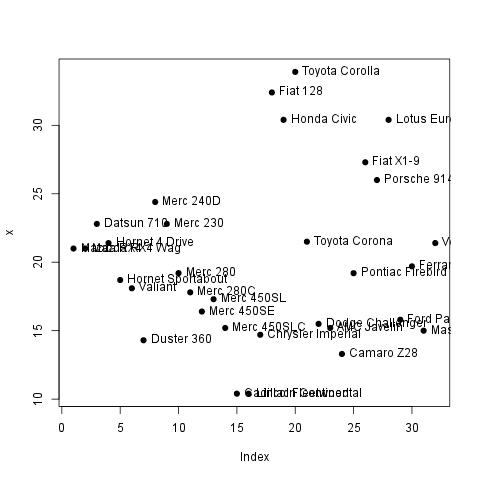
\includegraphics{KKORo27NO5ORo5llNoO38oO7e2OWO2IOO757OolWmlQ87hPGOlJeOjOv5om7NP7hPGOQ5ANQOjOo8RoI5HNOholoB575oGOl8OOjOto.png}
\caption{}
\end{figure}

So far we've been dealing with data.frames and plots, now let's deal
with variables

Now we'll see if the Z var is working properly. If I omit it, it should
perserve the default value (TRUE)\ldots{} aaaand\ldots{}. TRUE.

OK, so far, so good, but let's see what's going on with code
chunks\ldots{}

\ctable[pos = H, center, botcap]{llllllllll}
{% notes
}
{% rows
\FL
0.22234 & 0.65173 & 1.39133 & 0.98333 & --0.58344 & --0.99095 & --0.45373 & --0.65796 & 2.37939 & 2.06748
\\\noalign{\medskip}
--0.31492 & --0.84771 & --0.55026 & 0.91617 & --0.16968 & 1.27141 & 0.46340 & --0.10636 & --0.18371 & --0.24102
\\\noalign{\medskip}
0.07103 & 0.00653 & --0.35326 & 0.81124 & 0.17430 & --0.15579 & --0.14371 & 1.03454 & --0.11201 & 0.77493
\\\noalign{\medskip}
0.85391 & --1.71403 & 0.53827 & 0.22948 & 0.32925 & --0.39897 & 1.07016 & --1.15996 & --0.04254 & 0.99816
\\\noalign{\medskip}
1.84811 & --1.97597 & 1.90410 & 0.29464 & --0.26010 & 0.05813 & --1.38199 & 0.54703 & --0.05245 & 0.24624
\\\noalign{\medskip}
--0.74688 & 1.50558 & --0.13179 & 1.68098 & 1.29912 & 0.21735 & 0.89660 & 0.09138 & --0.31560 & 0.93897
\\\noalign{\medskip}
--1.55898 & 3.47041 & 1.33684 & 0.26634 & --0.14000 & 0.42141 & --0.14711 & --0.91866 & --1.73281 & 0.48034
\\\noalign{\medskip}
--1.08743 & --0.62727 & 0.58817 & --1.52503 & --0.61666 & 0.03544 & --0.87532 & 0.41800 & --0.49410 & --0.47320
\\\noalign{\medskip}
--0.14827 & --0.08834 & --1.65963 & 0.34622 & 0.59807 & 0.13834 & 0.62300 & 0.74279 & 0.71904 & 1.04388
\\\noalign{\medskip}
--0.65230 & --0.71892 & --2.85295 & 0.08785 & --0.30507 & --1.72776 & 0.76428 & 1.77922 & 1.05258 & 1.01411
\LL
}

When it comes to CSV values, let us see how do they work. You have
chosen the ``foo''.

\end{document}
